\documentclass[a4paper,12pt,oneside]{report}

\newif\ifrelease % new boolean variable release. True = include some fancy content
\releasefalse % and set it

\usepackage[english]{babel}
\usepackage[utf8]{inputenc}
\usepackage[T1]{fontenc}
\usepackage{amsmath}
\usepackage{amssymb}
\usepackage{epsfig}
\usepackage{graphicx}
\ifrelease
	\usepackage{pdfpages}
\fi
\usepackage[pagebackref=true]{hyperref} % tento balicek by mel byt na konci baliku!

\hypersetup{
	pdfauthor={Matej Laitl},
	pdftitle={Implementation environment for Bayesian filtering algorithms}
}

%% Nastavení zrcadla sazby
\usepackage{calc}
\setlength{\textheight}{9in}
\setlength{\textwidth}{6in}
\setlength\oddsidemargin{(\paperwidth-\textwidth)/2 - 1in}
\setlength\evensidemargin{(\paperwidth-\textwidth)/2 - 1in}
\setlength\topmargin{(\paperheight-\textheight-\headheight-\headsep-\footskip)/2 - 1in}

%\parindent=0pt % odsazení 1. řádku odstavce
\parskip=4pt   % mezera mezi odstavci

\ifrelease
	\hypersetup{pdfborder={0 0 0}} % no borders around links
\else
	\hypersetup{colorlinks=true} % colour links instead of borders
\fi

% definitions of our own commands:
\newcommand{\pdf}{probability density function}
\newcommand{\pdfs}{probability density functions}
\newcommand{\supp}{\operatorname{supp}}
\newcommand{\assign}{\leftarrow} % TODO: what symbol to use in formulas for assignment? =, := or <-?


\begin{document}

\ifrelease
	\newcommand{\cvut}{České vysoké učení technické v~Praze}
\newcommand{\fjfi}{Fakulta jaderná a fyzikálně inženýrská}
\newcommand{\km}{Katedra matematiky}
\newcommand{\obor}{Inženýrská Informatika}
\newcommand{\zamereni}{Softwarové inženýrství a matematická informatika}

\newcommand{\nazevcz}{Prostředí pro implementaci algoritmů Bayesovské filtrace}
\newcommand{\nazeven}{Implementation environment for Bayesian filtering algorithms}
\newcommand{\autor}{Matěj Laitl}
\newcommand{\rok}{2011}
\newcommand{\vedouci}{Ing. Václav Šmídl, Ph.D.}

\newcommand{\pracovisteVed}{Oddělení adaptivních systémů \\
	Ústav teorie informace a automatizace \\
	Akademie věd České republiky}
\newcommand{\konzultant}{---}
\newcommand{\pracovisteKonz}{}

\newcommand{\klicova}{Bayesovská filtrace, softwarová analýza, Python, Cython} % TODO: dalsi?
\newcommand{\keyword}{Bayesian filtering, software analysis, Python, Cython}
% Abstrakt práce: (cca 7 vět, min. 80 slov)
\newcommand{\abstrCZ}{Bayesovská filtrace je velmi použitelný přístup k odhadování dynamických
systémů, který má mnoho aplikací v robotice, environmentálních simulacích a dalších oborech. Tato
práce předkládá popis Kalmanova filtru, částicového filtru a marginalizovaného částicového filtru,
který využívá myšlenky obou předchozích. Poté je provedena softwarová analýza, která má za úkol
určit nejvhodnější implementační prostředí pro softwarovou knihovnu poskytující metody Bayesovské
filtrace. Nejprve jsou posouzeny obecné přístupy k vývoji software, z nichž je jako nejpoužitelnější
zvolen objektově orientovaný, následuje porovnání programovacích jazyků C++, MATLAB a Python.
Python zvítězí a v je něm napsána knihovna pro Bayesovskou filtraci nazvaná PyBayes; nakonec je
dosaženo výrazného zrychlení Pythonového kódu použitím Cythonu.}
\newcommand{\abstrEN}{Bayesian filtering is a vital approach to dynamic system estimation that has
wide applications in robotics, environmental simulations and much more. This text briefly introduces
the Kalman filter, the particle filter and the marginalized particle filter which combines ideas of
both. Software analysis is performed with the aim to identify the most suitable implementation
environment for a software library for Bayesian filtering. Various paradigms of software development
and are discussed among which the object-oriented programming is chosen; C++, MATLAB and Python
languages are evaluated. Python is determined most appropriate and a Python software library named
PyBayes is developed; dramatic performance gains are measured when Cython is used to speed up
Python.}

%%% zde zacina kresleni dokumentu

% titulní strana
\thispagestyle{empty}

\begin{center}
	{\Large  \bf  \cvut\\[2mm] \fjfi }
	\vspace{10mm}

	\begin{tabular}{c}
	{\bf \km}\\
	{\bf Obor: \obor}\\
	{\bf Zaměření: \zamereni}
	\end{tabular}

	\vspace{10mm} \epsfysize=20mm  \epsffile{cvut-logo-bw-600} \vspace{15mm}

	{\LARGE
	\textbf{\nazevcz}
	\par}

	\vspace{5mm}

	{\LARGE
	\textbf{\nazeven}
	\par}

	\vspace{30mm}
	{\Large BAKALÁŘSKÁ PRÁCE}

\end{center}

\vfill
{\large
\begin{tabular}{rl}
Vypracoval: & \autor\\
Vedoucí práce: & \vedouci\\
Rok: & \rok
\end{tabular}
}

% zadání bakalářské práce
\newpage
\thispagestyle{empty} Před svázáním místo téhle stránky \fbox{vložíte zadání práce} s podpisem
děkana (bude to jediný oboustranný list ve Vaší práci) !!!!

% prohlášení
\newpage
\thispagestyle{empty}
~
\vfill


{\bf Prohlášení}

\vspace{0.5cm}
Prohlašuji, že jsem svou bakalářskou práci vypracoval samostatně a použil jsem pouze podklady
(literaturu, projekty, SW atd.) uvedené v přiloženém seznamu.

\vspace{5mm}V Praze dne ....................\hfill
    \begin{tabular}{c}
    ........................................\\
    \autor
    \end{tabular}

% poděkování
\newpage
\thispagestyle{empty}
~
\vfill

{\bf Poděkování}

\vspace{5mm}
Děkuji Ing. Václavu Šmídlovi, Ph.D. za vedení mé bakalářské práce, velmi prozíravě položené
softwarové otázky a za poukázání na softwarové projekty (Cython, Sphinx, \ldots), které se ukázaly
být klíčové pro moji bakalářskou práci a softwarový projekt.

\begin{flushright}
\autor
\end{flushright}

% strana s abstraktem
\newpage
\thispagestyle{empty}

\newbox\odstavecbox
\newlength\vyskaodstavce
\newcommand\odstavec[2]{%
    \setbox\odstavecbox=\hbox{%
         \parbox[t]{#1}{#2\vrule width 0pt depth 4pt}}%
    \global\vyskaodstavce=\dp\odstavecbox
    \box\odstavecbox}
\newcommand{\delka}{120mm}

\noindent\begin{tabular}{@{}ll}
  {\em Název práce:} & ~ \\
  \multicolumn{2}{@{}l}{\odstavec{\textwidth}{\bf \nazevcz}} \\[5mm]
  {\em Autor:} & \autor \\[5mm]
  {\em Obor:} & \obor \\
  {\em Druh práce:} & Bakalářská práce \\[5mm]
  {\em Vedoucí práce:} & \odstavec{\delka}{\vedouci \\ \pracovisteVed} \\[5mm]
  {\em Konzultant:} & \odstavec{\delka}{\konzultant \\ \pracovisteKonz} \\[5mm]
  \multicolumn{2}{@{}l}{\odstavec{\textwidth}{{\em Abstrakt:} ~ \abstrCZ \\ }} \\[5mm]
  {\em Klíčová slova:} & \odstavec{\delka}{\klicova} \\[10mm]

  {\em Title:} & ~\\
  \multicolumn{2}{@{}l}{\odstavec{\textwidth}{\bf \nazeven}}\\[5mm]
  {\em Author:} & \autor \\[5mm]
  \multicolumn{2}{@{}l}{\odstavec{\textwidth}{{\em Abstract:} ~ \abstrEN \\ }} \\[5mm]
  {\em Key words:} & \odstavec{\delka}{\keyword}
\end{tabular}
 % include some fancy start pages
\fi


% obsah
\newpage
\tableofcontents


\chapter*{Notation} \addcontentsline{toc}{chapter}{Notation}

Throughout this text, following notation is used

\bigskip

\begin{tabular}{l p{0.8\textwidth}}
	\(\mathbb{N}\) & set of natural numbers \\
	\(\mathbb{R}\) & set of real numbers \\
	\(t\) & discrete time moment; \(t \in \mathbb{N}\) \\
	\(a_t\) & value of quantity \(a\) at time \(t\); \(a_t \in \mathbb{R}^n, n \in \mathbb{N}\) \\
		& unless noted otherwise, \(x_t\) denotes state vector at time \(t\) and \(y_t\) denotes
		  observation vector at time \(t\) \\
	\(a_{i:j}\) & sequence of quantities \((a_i, a_{i+1} \dots a_{j-1}, a_j)\) \\
	\(\mathcal{N}(\mu, \Sigma)\) & multivariate normal (Gaussian) probability density
		function{\footnotemark} with mean vector \(\mu\) and covariance matrix \(\Sigma\) \\
\end{tabular}

% \footnote does not work in tabular env, - this can be worked around with this
\footnotetext{for the purpose of this text, {\pdf} \(p\) is multivariate non-negative function
\(\mathbb{R}^n \rightarrow \mathbb{R}; \; \int_{\supp p} p(x_1, x_2 \dots x_n) \; \mathrm{d} x_1 x_2 \dots x_n = 1\)}


\chapter*{Introduction} \addcontentsline{toc}{chapter}{Introduction}

TODO motivatin for bayes filtration + a need for a convenient library (rapid prototyping vs. speed)

applications: robotics, navigation, + tracking of toxic plume after radiation accident.

Decision-making being a logical and natural ``next step'' - beyond the scope of this text.

[proposed citations:\cite{ThrBurFox:05,Gus:02,HofSmi:09,HofSmiPech:09,PechHofSmi:09}]


\chapter{Basics of Recursive Bayesian Estimation}

In following sections the problem of recursive Bayesian estimation is stated and its analytical
solution is derived. Later on, due to practical intractability of the solution in its general form,
a few methods that either simplify the problem or approximate the solution are shown.

\section{Problem Statement}

Assume a dynamic system described by a hidden real-valued \emph{state vector} \(x\) which evolves at
discrete time steps according to a known function \(f_t\) (in this text called \emph{process model})
as described by \eqref{eq:DynSysFt}.
\begin{equation} \label{eq:DynSysFt}
	x_t = f_t(x_{t-1}, v_{t-1})
\end{equation}

Variable \(v_t\) in \eqref{eq:DynSysFt} denotes random \emph{process noise}, which may come from various
sources and is often inevitable. Sequence of \(v_t\) is assumed to be identically independently
distributed random variable sequence.

The state of the system is hidden and can only be observed though a real-valued \emph{observation vector}
\(y\) that relates to the state \(x\) as in \eqref{eq:DynSysHt}, but adds further \emph{observation
noise} \(w\).
\begin{equation} \label{eq:DynSysHt}
	y_t = h_t(x_t, w_t)
\end{equation}

In \eqref{eq:DynSysHt} \(h_t\) is known function called \emph{observation model} in this text and \(w_t\) is
identically independently distributed random variable sequence that denotes observation noise.

The goal of recursive\footnote{by the word recursive we mean that it is not needed to keep track of
the whole batch of previous observations in practical methods, only appropriate quantities from time
moments \(t-1\) and \(t\) are needed to estimate \(x_t\). However, this does not apply to the
derivation of the solution, where the notation of whole batch of observations \(y_{1:t}\) is used.}
Bayesian estimation is to give an estimate of the state \(x_t\) given the
observations \(y_{1:t}\) provided the knowledge of the functions \(f_t\) and \(h_t\).
More formally, the goal is to find the {\pdf} \(p(x_t | y_{1:t})\).
Theoretical solution to this problem is known and is presented in next section.

\section{Theoretical solution}

At first, we observe that {\pdf} \(p(x_t|x_{t-1})\) can be derived from the process model
\eqref{eq:DynSysFt} (given the distribution of \(v_k\)) and that \(p(y_t|x_t)\) can be derived from
the observation model \eqref{eq:DynSysHt} respectively. (given the distribution of \(w_k\))

Because recursive solution is requested, suppose that \(p(x_{t-1}|y_{1:t-1})\) and
\(p(x_0)\) are known\footnote{\(p(x_0)\) is known as the initial {\pdf} of the state vector} in
order to be able to make the transition \(t-1 \; \rightarrow \; t\).

In the first stage that can be called \emph{prediction}, \emph{a priori} {\pdf}
\(p(x_t | y_{1:t-1})\) is calculated without knowledge of \(y_t\). We begin the derivation by
performing the reverse of the marginalization over \(x_{k-1}\).
\begin{equation*}
	p(x_t | y_{1:t-1}) = \int_{-\infty}^{\infty} p(x_t, x_{t-1} | y_{1:t-1}) \; \mathrm{d} x_{t-1}
\end{equation*}

Using chain rule for {\pdfs}, the element of integration can be split.
\begin{equation*}
	p(x_t | y_{1:t-1}) = \int_{-\infty}^{\infty} p(x_t | x_{t-1}, y_{1:t-1}) p(x_{t-1} | y_{1:t-1}) \; \mathrm{d} x_{t-1}
\end{equation*}

With an assumption that the modelled dynamic system \eqref{eq:DynSysFt} possesses
\emph{Markov Property}, \(p(x_t | x_{t-1}, y_{1:t-1})\) equals \(p(x_t | x_{t-1})\).~\cite{AruMasGor:02}
This leaves us with the result \eqref{eq:APrioriPdf}.
\begin{equation} \label{eq:APrioriPdf}
	p(x_t | y_{1:t-1}) = \int_{-\infty}^{\infty} p(x_t | x_{t-1}) p(x_{t-1} | y_{1:t-1}) \; \mathrm{d} x_{t-1}
\end{equation}

As we can see, a priori {\pdf} only depends on previously known functions and therefore can be
calculated.

We continue with the second stage that could be named \emph{update}, where new observation \(y_t\) is taken into
account and \emph{a posteriori} {\pdf} \(p(x_t | y_{1:t})\) is calculated. Bayes' theorem can be used
to derive a posteriori {\pdf} \eqref{eq:APosterioriPdfRaw}.
\begin{equation} \label{eq:APosterioriPdfRaw}
	p(x_t | y_{1:t}) = \frac{p(y_t | x_t, y_{1:t-1}) p(x_t | y_{1:t-1})}{p(y_t | y_{1:t-1})}
\end{equation}

According to the observation model \eqref{eq:DynSysHt} and assuming Markov property, \(y_t\) only
depends on \(x_t\). That is \(p(y_t | x_t, y_{1:t-1}) = p(y_t | x_t)\). Therefore a posteriori
{\pdf} can be further simplified into \eqref{eq:APosterioriPdf}.
\begin{equation} \label{eq:APosterioriPdf}
	p(x_t | y_{1:t}) = \frac{p(y_t | x_t) p(x_t | y_{1:t-1})}{p(y_t | y_{1:t-1})}
\end{equation}

While both {\pdfs} in the numerator of \eqref{eq:APosterioriPdf} are already known, \(p(y_t|y_{1:t-1})\)
found in the denominator can be calculated using the formula \eqref{eq:MargLikelihood}, where
marginalization over \(x_t\) is preformed. Quantity \eqref{eq:MargLikelihood} can also be interpreted as
\emph{marginal likelihood} (sometimes called \emph{evidence}) of observation.~\cite{Smi:10}
\begin{equation} \label{eq:MargLikelihood}
	p(y_t | y_{1:t-1}) = \int_{-\infty}^{\infty} p(y_t | x_t) p(x_t | y_{1:t-1}) \; \mathrm{d} x_{t}
\end{equation}

Computing \eqref{eq:MargLikelihood} isn't however strictly needed as it does not depend on \(x_t\) and
serves as a normalising constant in \eqref{eq:APosterioriPdf}. Depending on use-case the normalising
constant may not be needed at all or may be computed alternatively using the fact that \(p(x_t | y_{1:y})\)
integrates to \(1\).

We have shown that so called \emph{optimal Bayesian solution}\cite{AruMasGor:02} can be easily
analytically inferred using only \emph{chain rule for {\pdfs}}, \emph{marginalization} and
\emph{Bayes' theorem}. (equations \eqref{eq:APrioriPdf}, \eqref{eq:APosterioriPdf} and
\eqref{eq:MargLikelihood} forming the main steps of the solution) On the other hand, using this
method directly in practice proves difficult because at least one parametric multidimensional
integration has to be performed (in \eqref{eq:APrioriPdf}), which is (in its general form) hardly
tractable for greater than small state vector dimensions.

This is a motivation for various simplifications and approximations among which we have chosen
Kalman filter described in the next section and particle filter family described later.

\section{Kalman Filter}

Kalman filter\footnote{first presented by Rudolf Emil Kalman in 1960} poses additional set of strong
assumptions on modelled dynamic system, but greatly
simplifies optimal Bayesian solution \eqref{eq:APrioriPdf}, \eqref{eq:APosterioriPdf} into a
sequence of algebraic operations with matrices. On the other hand, when these requirements can be
fulfilled, there is no better estimator in Bayesian point of view because Kalman filter computes
\(p(x_t | y_{1:t})\) \emph{exactly}\footnote{not accounting for numeric errors that arise in
practical implementations}.

Assumptions additionally posed on system by Kalman filter are: % TODO: I don't want space between this and enumeration!
\begin{enumerate}
	\item \(f_t\) in the process model \eqref{eq:DynSysFt} is a linear function of \(x_t\) and
	\(v_t\).
	\item \(v_t \sim \mathcal{N}(0, Q_t)\) meaning that process noise \(v_t\) is normally
	distributed with zero mean\footnote{zero mean assumption is not strictly needed, it is however
	common in many implementations.} and with known covariance matrix \(Q_t\).
	\item \(h_t\) in the observation model \eqref{eq:DynSysHt} is a linear function of \(x_t\) and
	\(w_t\).
	\item \(w_t \sim \mathcal{N}(0, R_t)\) meaning that observation noise \(w_t\) is normally distributed
	with zero mean and with known covariance matrix \(R_t\).
	\item both initial state {\pdf} is Gaussian.
\end{enumerate}

It can be proved that if above assumptions hold, \(p(x_t|y_{1:t})\) is Gaussian for all
\(t > 0\).~\cite{AruMasGor:02} Furthermore, given assumptions 1. and 2. the process model
\eqref{eq:DynSysFt} can be reformulated as \eqref{eq:LinSysAt}, where \(A_t\) is real-valued matrix
that represents \(f_t\).
Using the same idea and assumptions 3. and 4. the observation model \eqref{eq:DynSysHt} can be
expressed as \eqref{eq:LinSysCt}, \(C_t\) being real-valued matrix representing \(h_t\). Another
common requirement used below in algorithm description is that \(v_t\) and \(w_t\) are
stochastically independent.
\begin{align}
	x_t &= A_t x_{t-1} + \hat{v}_{t-1} & A_t &\in \mathbb{R}^{n,n} \;\; n \in \mathbb{N} \label{eq:LinSysAt} \\
	y_t &= C_t x_t + \hat{w}_t & C_t &\in \mathbb{R}^{j,n} \;\; j \in \mathbb{N} \;\; j \leq n \label{eq:LinSysCt}
\end{align}

Note that we have marked noises \(v_t\) and \(w_t\) as \(\hat{v}_t\) and \(\hat{w}_t\) when they
are transformed through \(A_t\), respectively \(C_t\) matrix. Let also \(\hat{Q}_t\) denote the
covariance matrix of \(\hat{v}_t\) and \(\hat{R}_t\) denote the covariance matrix of \(\hat{w}_t\)
in further text.

At this point we can describe the algorithm of Kalman filter. As stated above, a posteriori {\pdf}
is Gaussian and thus can be parametrised by mean vector \(\mu\) and covariance matrix \(P\). Let us
denote a posteriori mean from previous iteration by \(\mu_{t-1|t-1}\) and associated covariance by
\(P_{t-1|t-1}\) as in \eqref{eq:KalmanPreAPost}.
\begin{equation} \label{eq:KalmanPreAPost}
	p(x_{t-1} | y_{1:t-1}) = \mathcal{N}(\mu_{t-1|t-1}, P_{t-1|t-1})
\end{equation}

A priori {\pdf} \eqref{eq:KalmanAPrior} can then be calculated as follows:~\cite{AruMasGor:02}
\begin{align}
	p(x_t | y_{1:t-1}) &= \mathcal{N}(\mu_{t|t-1}, P_{t|t-1}) \label{eq:KalmanAPrior} \\
	\mu_{t|t-1} &\assign A_t \mu_{t-1|t-1} \notag \\
	P_{t|t-1} &\assign A_t P_{t-1|t-1} A_t^T + \hat{Q}_{t-1} \notag
\end{align}

Before introducing a posteriori {\pdf} it is useful to establish another Gaussian {\pdf}
\eqref{eq:KalmanEvidence} that is not necessarily needed, but is useful because it represents
marginal likelihood \eqref{eq:MargLikelihood}. % TODO: right? citation for this!
[TODO: is that right? have to find citation (\cite{Smi:10} is general, but one that shows we can compute it this way for KF would be good)]
\begin{align}
	p(y_t|y_{1:t-1}) &= \mathcal{N}(\nu_{t|t-1}, S_{t|t-1}) \label{eq:KalmanEvidence} \\
	\nu_{t|t-1} &\assign C_t \mu_{t|t-1} \notag \\
	S_{t|t-1} &\assign C_t P_{t|t-1} C_t^T + \hat{R}_t \notag
\end{align}

The update phase of Kalman filter can be performed by computing so-called \emph{Kalman gain} matrix
\eqref{eq:KalmanGain}, a posteriori {\pdf} \eqref{eq:KalmanAPost} is then derived from a priori one
using Kalman gain \(K_t\) and observation \(y_t\).~\cite{AruMasGor:02}
\begin{align}
	K_t &\assign P_{t|t-1} C_t^T S_{t|t-1}^{-1} \label{eq:KalmanGain} \\[\parskip]
	p(x_t|y_{1:t}) &= \mathcal{N}(\mu_{t|t}, P_{t|t}) \label{eq:KalmanAPost} \\
	\mu_{t|t} &\assign \mu_{t|t-1} + K_t(y_t - \nu_{t|t-1}) \notag \\
	P_{t|t} &\assign P_{t|t-1} - K_t C_t P_{t|t-1} \notag
\end{align}

In all formulas above \(A^T\) denotes a transpose of matrix \(A\) and \(A^{-1}\) denotes inverse
matrix to \(A\). As can be seen, formulas \eqref{eq:APrioriPdf} and \eqref{eq:APosterioriPdf} have
been reduced to tractable algebraic operations, computing inverse matrix\footnote{it can be shown
that \(S_{t|t-1}\) is positive definite given that \(C_t\) is full-ranked,
therefore the inverse in \eqref{eq:KalmanGain} exists} being the most costly one.

It should be further noted that Kalman filter and described algorithm can be easily enhanced to
additionally cope with \emph{intervention} (or control) vector applied to the system, making it
suitable for the theory of decision-making. Numerous generalisations of Kalman filter exist, for
example \emph{extended Kalman filter} that relaxes the requirement of linear system by locally
approximating non-linear system with Taylor series. These are out of scope of this
text, but provide areas for subsequent consideration.

On the other hand, the assumption of Gaussian a posteriori {\pdf} cannot be easily overcome and for
systems that show out non-Gaussian distributions of state vector another approach have to be
taken.~\cite{AruMasGor:02} One such approach can be Monte Carlo-based \emph{particle filter}
presented in the next section.

\section{Particle Filter}

\section{Marginalized Particle Filter}


\chapter{Software analysis}

\section{Requirements}

Ideal library for Bayesian filtering would posses following properties...:

\section{Programming paradigms}

Interpreted vs. Compiled

Object-oriented, procedural and Functional

pass-by reference vs. copy-on-write (Matlab)

\section{Survey of Existing Libraries for Bayesian estimation/decision making}

Brief survey of existing libraries ... not fullfilling all requirements..

The need to implement a new one :-)

\section{C++}

BDM

 - advantages of C (speed, C prevalence (many optimised libraries, BLAS, LAPACK.., OpenMP)

 - disadvantages of C in our ``situation'' (steep learning curve, coplexity because of low-levelness
   high initial barriers (need to have compiler, libraries...), inconveniently long edit/build/test
   process)

\section{Matlab}

BDM (partially?)

 - advantages (popularity, existing toolboxes, rapid development (high-level)

 - disadv: strict copy-on-write, problematic object model (not in original design), difficulties
           interfacing existing C (F) code

\section{Python}

NumPy.... parallelisation (approaches, improvements in Py 3.2) - GIL.. Py3k

\section{Cython}

general info etc... extension types, building, ease of interfacing C (and F) code, .pxd files,
NumPy support

[citations:\cite{BehBraSel:09,Sel:09,BehBraCitDalSelSmi:11}]

\subsection{Gradual Optimisation}

how can optimisaion be approached (gradually) and why this approach is superior

integrate\_python\_cython example (``100x'' speedup for a special (very simple) case)

\subsection{Parallelisation}

integrate\_python\_cython patched with OpenMP (13x speedup in 16-core system)

prange CEP

\subsection{Pure Python mode}

About it and why it should be used in a hypothetical bayesian python library

\subsection{Limitations}

2 types:

	not-supported code (few cases, but bad, ongoing work)

	not-optimised code (much more work needed, but not hard to fix in most cases)

		- exception handling (functions returning void etc)

		- limitations of pure python mode in regards to traditional .pyx files

\section{Choice}

python/cython was choosen ...


\chapter{The PyBayes Library}

Introduction, general directions, future considerations

+ open development on github, open-source

\section{Interpreted and Compiled}

\section{Library Layout}

[proposed citation: \cite{Smi:05}]

\subsection{Random Variable Meta-representation}

Why it is needed (ref to ProdCPdf)

\subsection{Probability Density Functions}

Nice UML diagrams! (better more smaller UMLs than one big) One for general pdf layut, one for
AbstractGaussPdf family, one for AbstractEmpPdf family

\subsection{Bayesian Filters}

UML

Nice graph of a run of a particle filter (Mirda has the plotting code)

similar of marginalized particle filter? (gausses would be plotted vertically)

[mention this:\cite{Smi:10}]

\section{Documentation, Testing and Profiling}

TODO: move above Library Layout?

Documenting using Sphinx, approach to documentation (mathematician-oriented), math in documentation

Testing - the separation of

- tests: test one class in isolation, quick, determinism (would be good, not achievable)

- stresses: test a great portion of code at once, run longer, non-determinism..

Profiling python/cython - how, existing support in PyBayes

- how to correct profiling-induced overhead

\section{Comparison with BDM}


\chapter*{Conclusion} \addcontentsline{toc}{chapter}{Conclusion}


% použitá literatura
\clearpage % so that the contents link mentions correct page
\phantomsection % so that hyperref makes correct reference
\addcontentsline{toc}{chapter}{\bibname}
\bibliographystyle{plain}
\bibliography{bibliography}

\ifrelease
	% přílohy
	\appendix % aby LaTeX cisloval jinak
	\clearpage % so that the contents link mentions correct page
	\phantomsection % so that hyperref makes correct reference
	\addcontentsline{toc}{chapter}{\appendixname}

	\part*{\appendixname}

	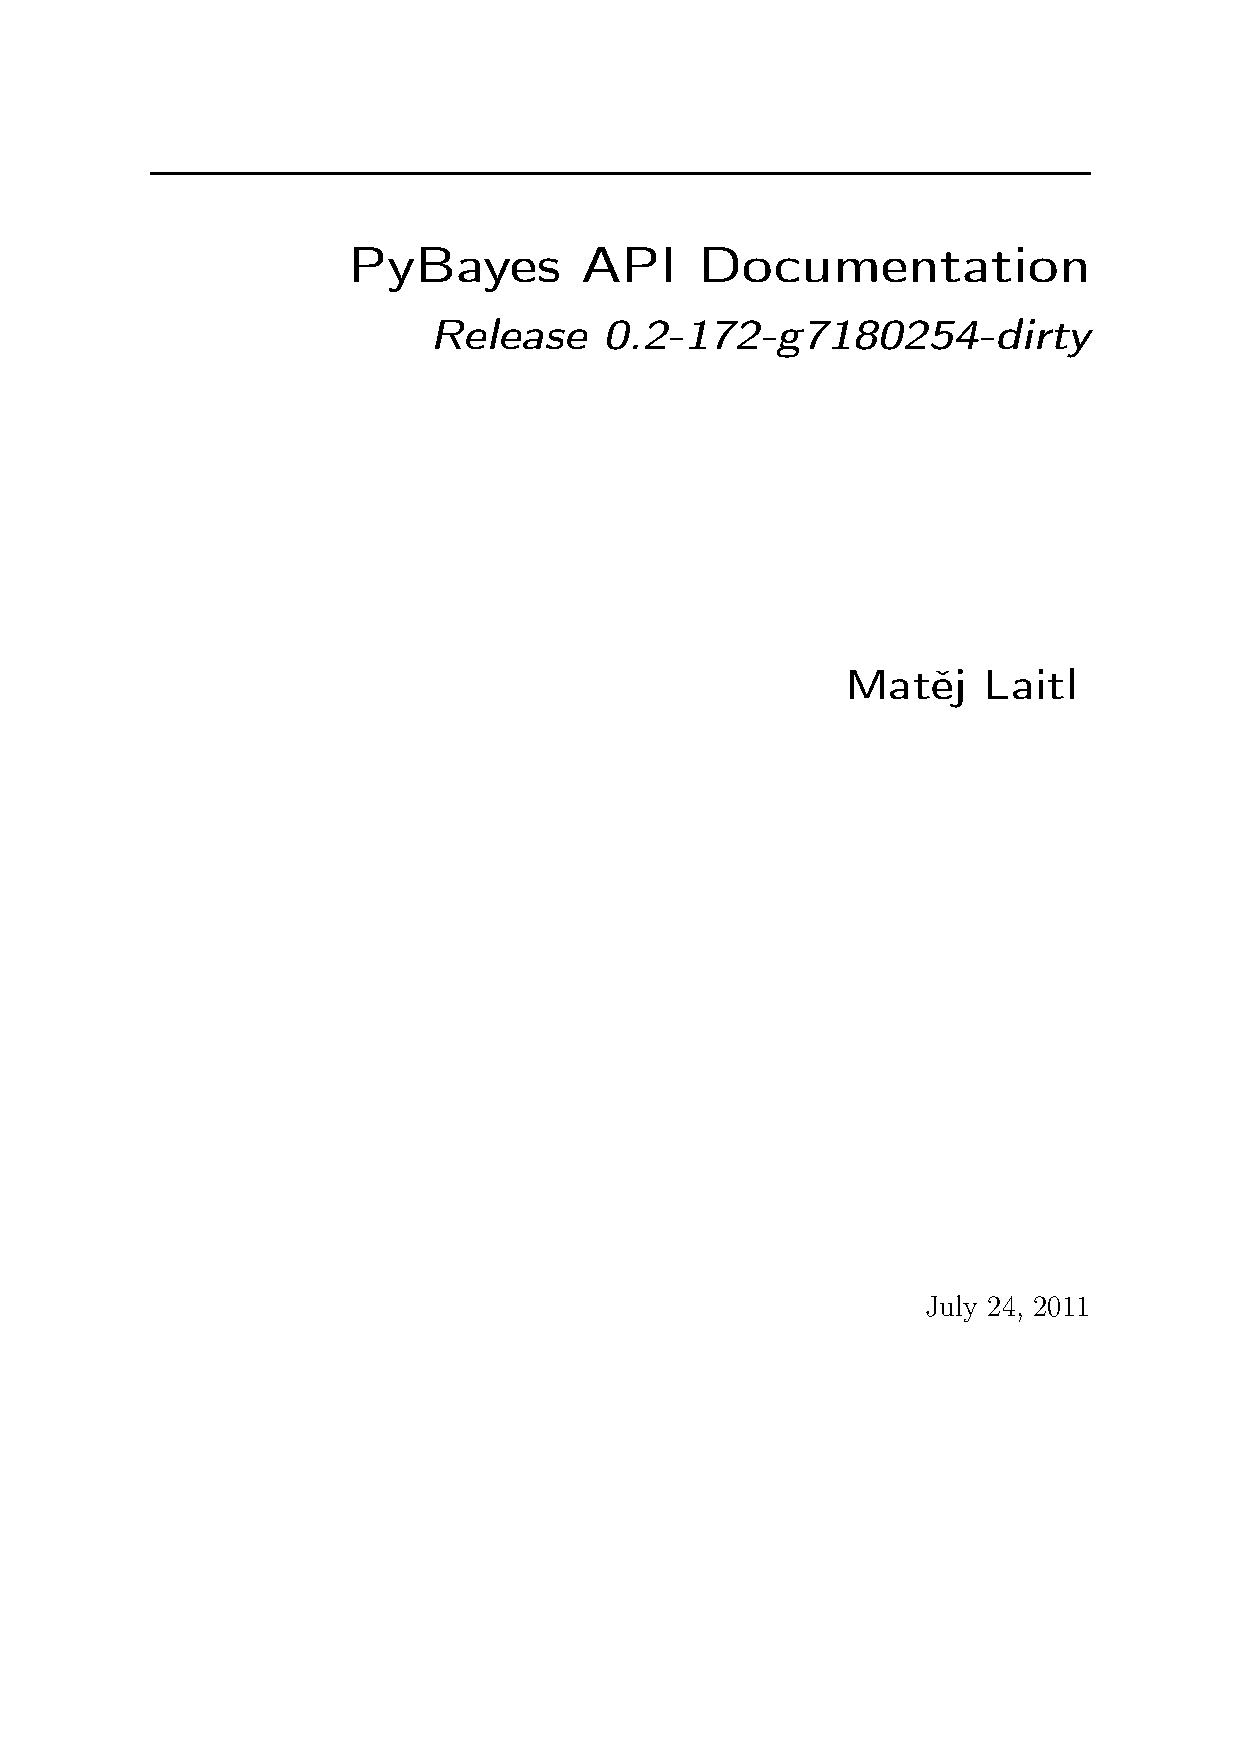
\includepdf[pages=-]{../doc/_build/latex/PyBayes.pdf}
\fi

\end{document}
